% 03_lab1_view
\newpage
\section{Основная часть}
\subsection{Лабораторная работа №1. Представления}
Задачи к лабораторной работе №1:
\begin{enumerate}
    \item Создать представление.
    \item Выполнить простой запрос к созданному представлению.
    \item Выполнить сложный запрос с присоединением к представлению других таблиц.
    \item Проверить обновляемость представления.
\end{enumerate}

\subsubsection{Создание представления}
Запрос, на основе которого было создано представление: для каждого студента подсчитать количество поселений и количество выполненных платежей. Код представления приведен в листинге~\ref{lst:create-view}.
\begin{lstlisting} [
    language=SQL,
    caption={Создание представления},
    label={lst:create-view}
]
CREATE VIEW student_settlement_payment_counts AS
SELECT
    student.student_id,
    student.last_name,
    student.first_name,
    student.middle_name,
    COUNT(DISTINCT settlement.settlement_id) AS settlement_count,
    COUNT(DISTINCT payment.payment_id) AS payment_count
FROM
    student
    LEFT JOIN settlement ON student.student_id = settlement.student_id
    LEFT JOIN payment ON settlement.settlement_id = payment.settlement_id
GROUP BY
    student.student_id,
    student.last_name,
    student.first_name,
    student.middle_name;
\end{lstlisting}

\subsubsection{Запросы}
Был составлен запрос, который выводит студентов, у которых количество выполненных платежей меньше, чем у студента «А». В результирующей таблице было выведено 4462 строк. Код запроса представлен в листинге~\ref{lst:view-query1}. Результирующая таблица представлена в таблице~\ref{tab:view-query1}. Графическое представление запроса приведено на рисунке~\ref{fig:view_query1}.
\begin{lstlisting} [
    language=SQL,
    caption={Простой запрос к представлению},
    label={lst:view-query1}
]
SELECT
    student_settlement_payment_counts.last_name,
    student_settlement_payment_counts.first_name,
    student_settlement_payment_counts.middle_name,
    student_settlement_payment_counts.settlement_count,
    student_settlement_payment_counts.payment_count
FROM
    student_settlement_payment_counts
WHERE
    student_settlement_payment_counts.payment_count < (
        SELECT
            payment_count
        FROM
            student_settlement_payment_counts
        WHERE
            last_name = 'Glover'
            AND first_name = 'Nels'
            AND middle_name = 'Aimee'
    )
ORDER BY
    settlement_count DESC,
    payment_count DESC;
\end{lstlisting}

\begin{table}[H]
    \centering
    \caption{Результат простого запроса}
    \label{tab:view-query1}
    \small
    \begin{tabular}{llllrr}
        \toprule
        Фамилия & Имя & Отчество & Поселения & Платежи \\
        \midrule
        Ankunding   & Mina       & Krystina  & 10 & 122 \\
        Schroeder   & Jamarcus   & Orval     & 10 & 122 \\
        Beahan      & Mertie     & Trey      & 10 & 122 \\
        Bogan       & Clifton    & Yasmine   & 10 & 122 \\
        Bosco       & Dannie     & Jalen     & 10 & 122 \\
        Langosh     & Orion      & Adrienne  & 10 & 122 \\
        Harris      & Hollie     & Harley    & 10 & 122 \\
        Lynch       & Winfield   & Quinton   & 10 & 122 \\
        \bottomrule
    \end{tabular}
\end{table}

\begin{figure}[H]
    \centering
    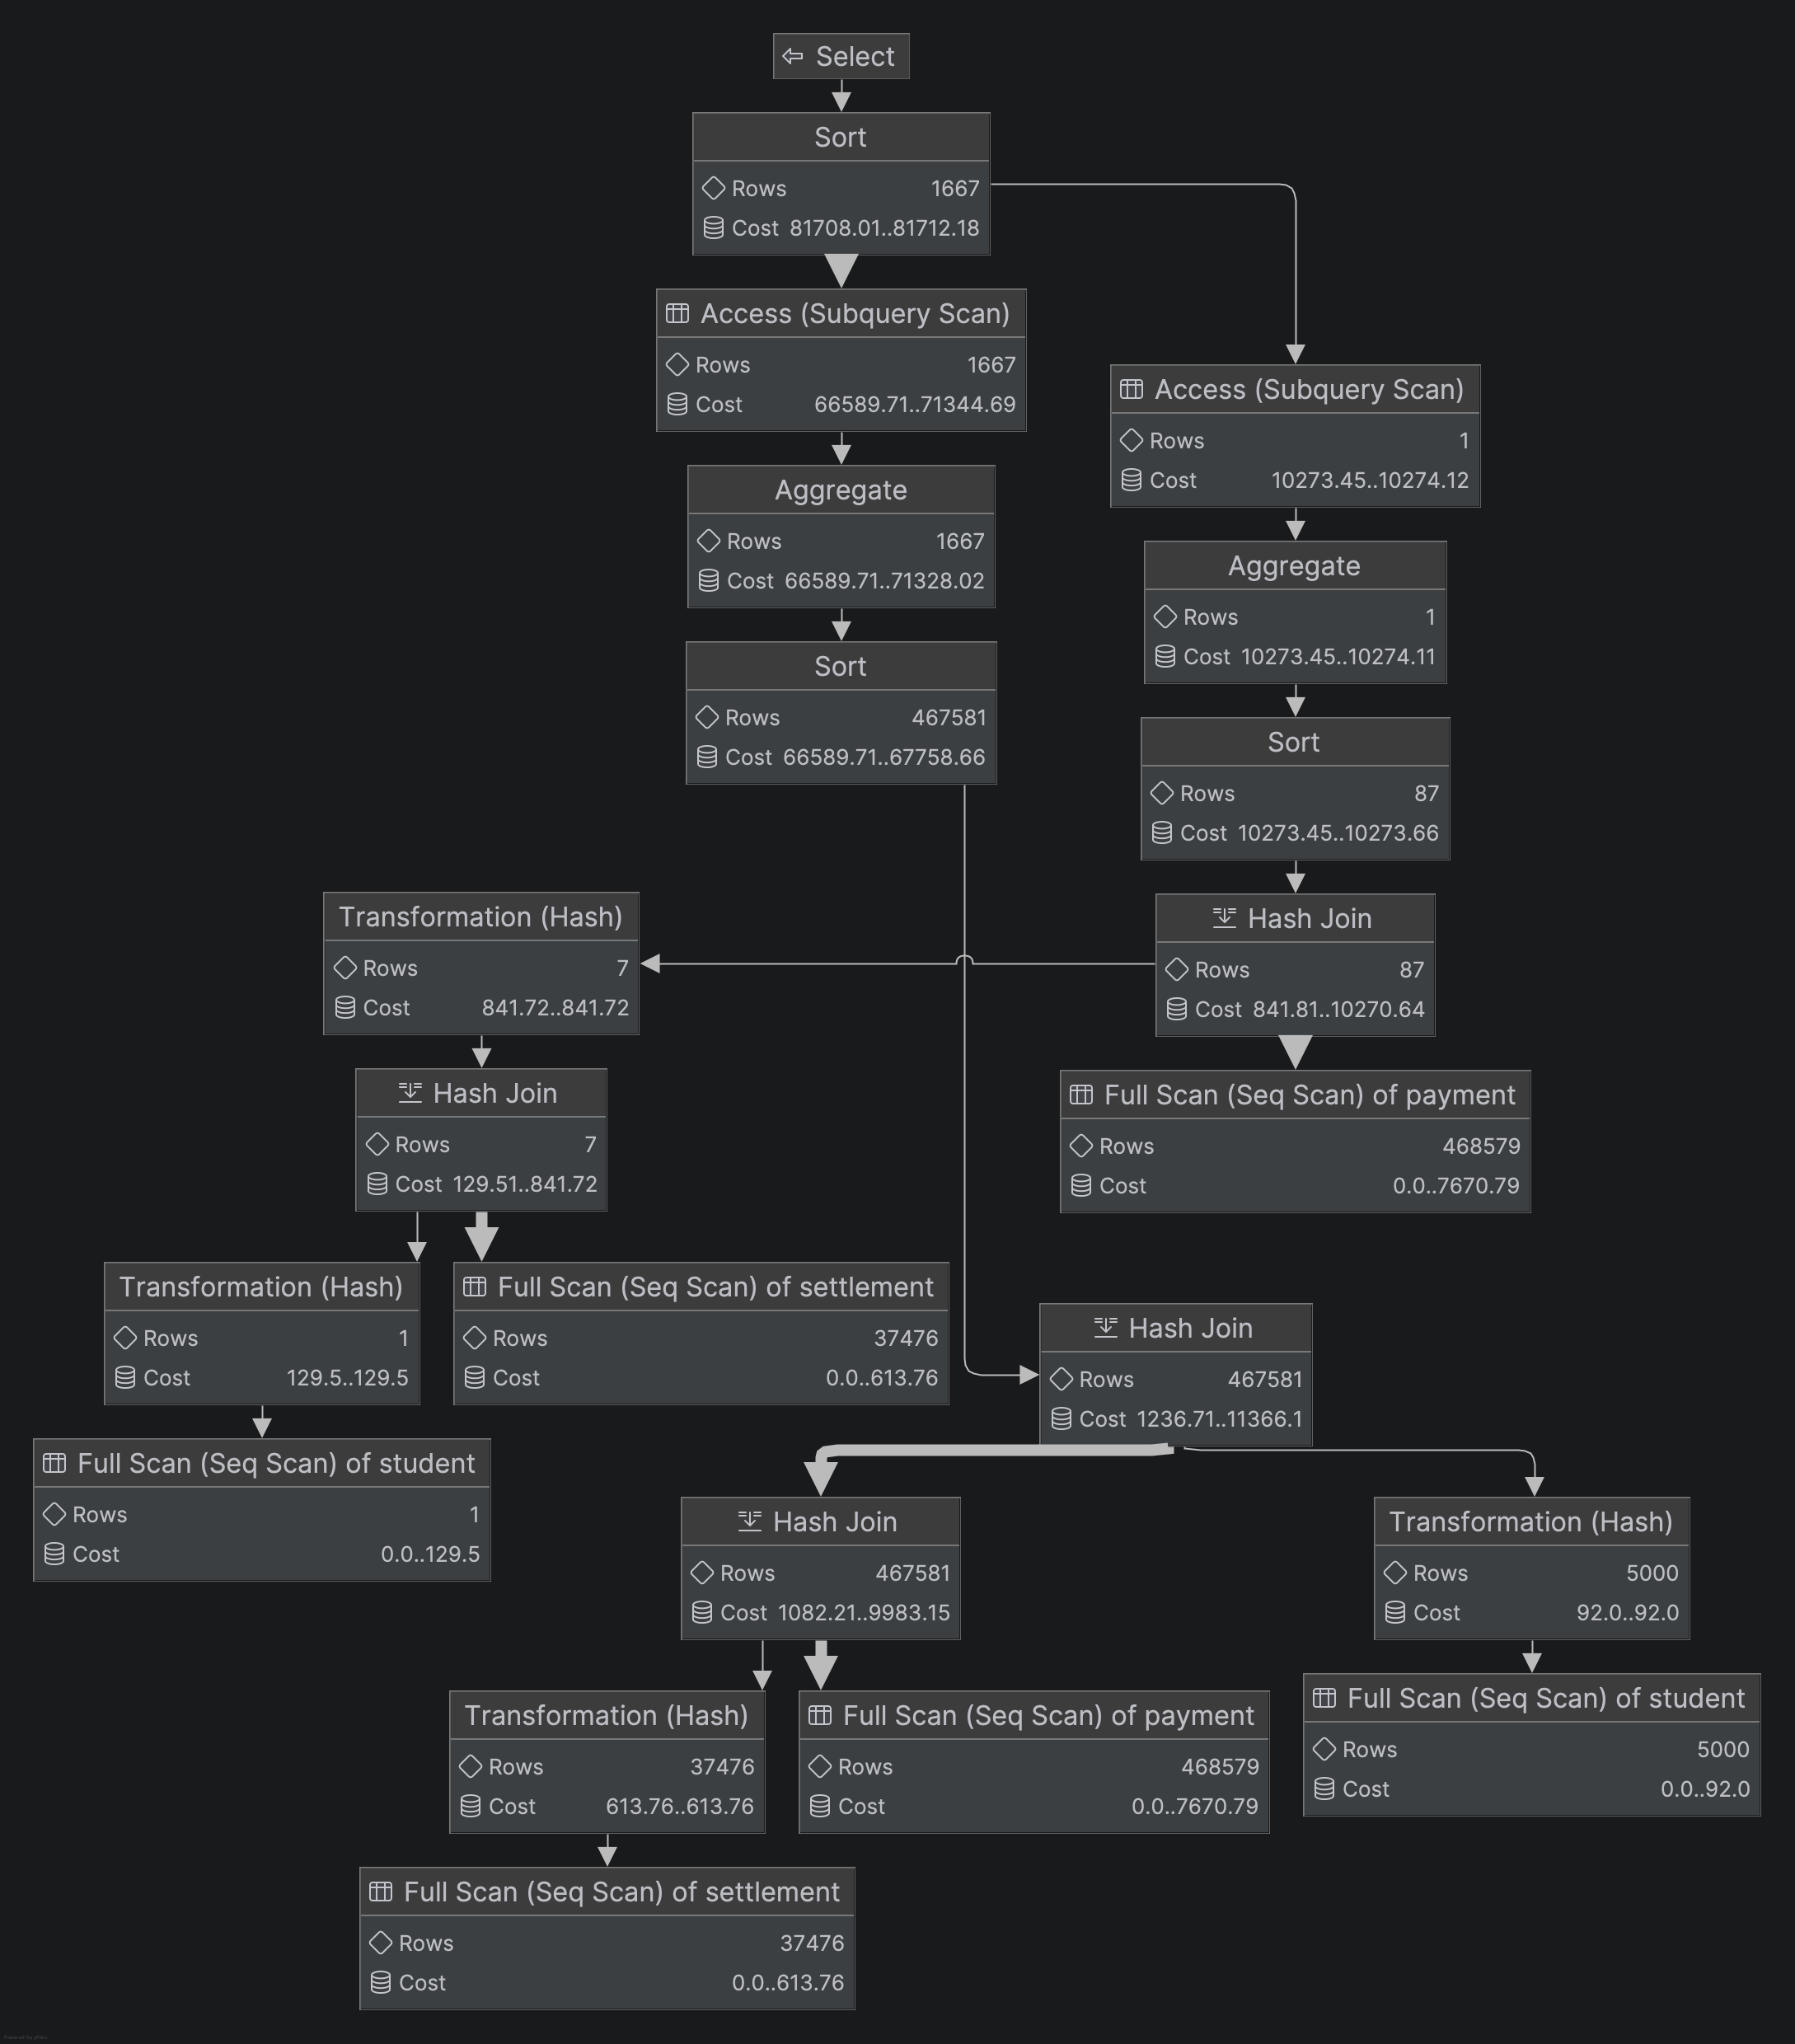
\includegraphics[width=0.8\textwidth]{figures/view_query1.png}
    \caption{Графическое представление простого запроса}
    \label{fig:view_query1}
\end{figure}

Далее был составлен сложный запрос, в котором осуществляется присоединение таблиц settlement и review. Запрос выводит для каждого студента количество поселений, количество платежей и количество отзывов. В результирующей таблице было выведено 5000 строк. Код запроса представлен в листинге~\ref{lst:view-query2}. Результирующая таблица представлена в таблице~\ref{tab:view-query2}. Графическое представление запроса приведено на рисунке~\ref{fig:view_query2}.
\begin{lstlisting} [
    language=SQL,
    caption={Сложный запрос к представлению},
    label={lst:view-query2}
]
SELECT
    student_settlement_payment_counts.last_name,
    student_settlement_payment_counts.first_name,
    student_settlement_payment_counts.middle_name,
    student_settlement_payment_counts.settlement_count,
    student_settlement_payment_counts.payment_count,
    COUNT(DISTINCT review.review_id) AS review_count
FROM
    student_settlement_payment_counts
    LEFT JOIN settlement ON settlement.student_id = student_settlement_payment_counts.student_id
    LEFT JOIN review ON review.settlement_id = settlement.settlement_id
GROUP BY
    student_settlement_payment_counts.student_id,
    student_settlement_payment_counts.last_name,
    student_settlement_payment_counts.first_name,
    student_settlement_payment_counts.middle_name,
    student_settlement_payment_counts.settlement_count,
    student_settlement_payment_counts.payment_count;
\end{lstlisting}

\begin{table}[H]
    \centering
    \caption{Результат сложного запроса}
    \label{tab:view-query2}
    \small
    \begin{tabular}{llllrrr}
        \toprule
        Фамилия & Имя & Отчество & Поселений & Платежей & Отзывов \\
        \midrule
        Glover      & Nels        & Aimee      & 10 & 123 & 47 \\
        Predovic    & Anastasia   & Christiana & 6  & 78  & 33 \\
        Eichmann    & Meredith    & Bernard    & 8  & 102 & 53 \\
        Blanda      & Greyson     & Kendrick   & 5  & 65  & 23 \\
        Legros      & Hillary     & Lillian    & 9  & 112 & 41 \\
        Jakubowski  & Lysanne     & Norberto   & 7  & 97  & 25 \\
        Daniel      & Donnell     & Syble      & 9  & 114 & 40 \\
        Mann        & Dayne       & Marina     & 5  & 58  & 42 \\
        \bottomrule
    \end{tabular}
\end{table}

\begin{figure}[H]
    \centering
    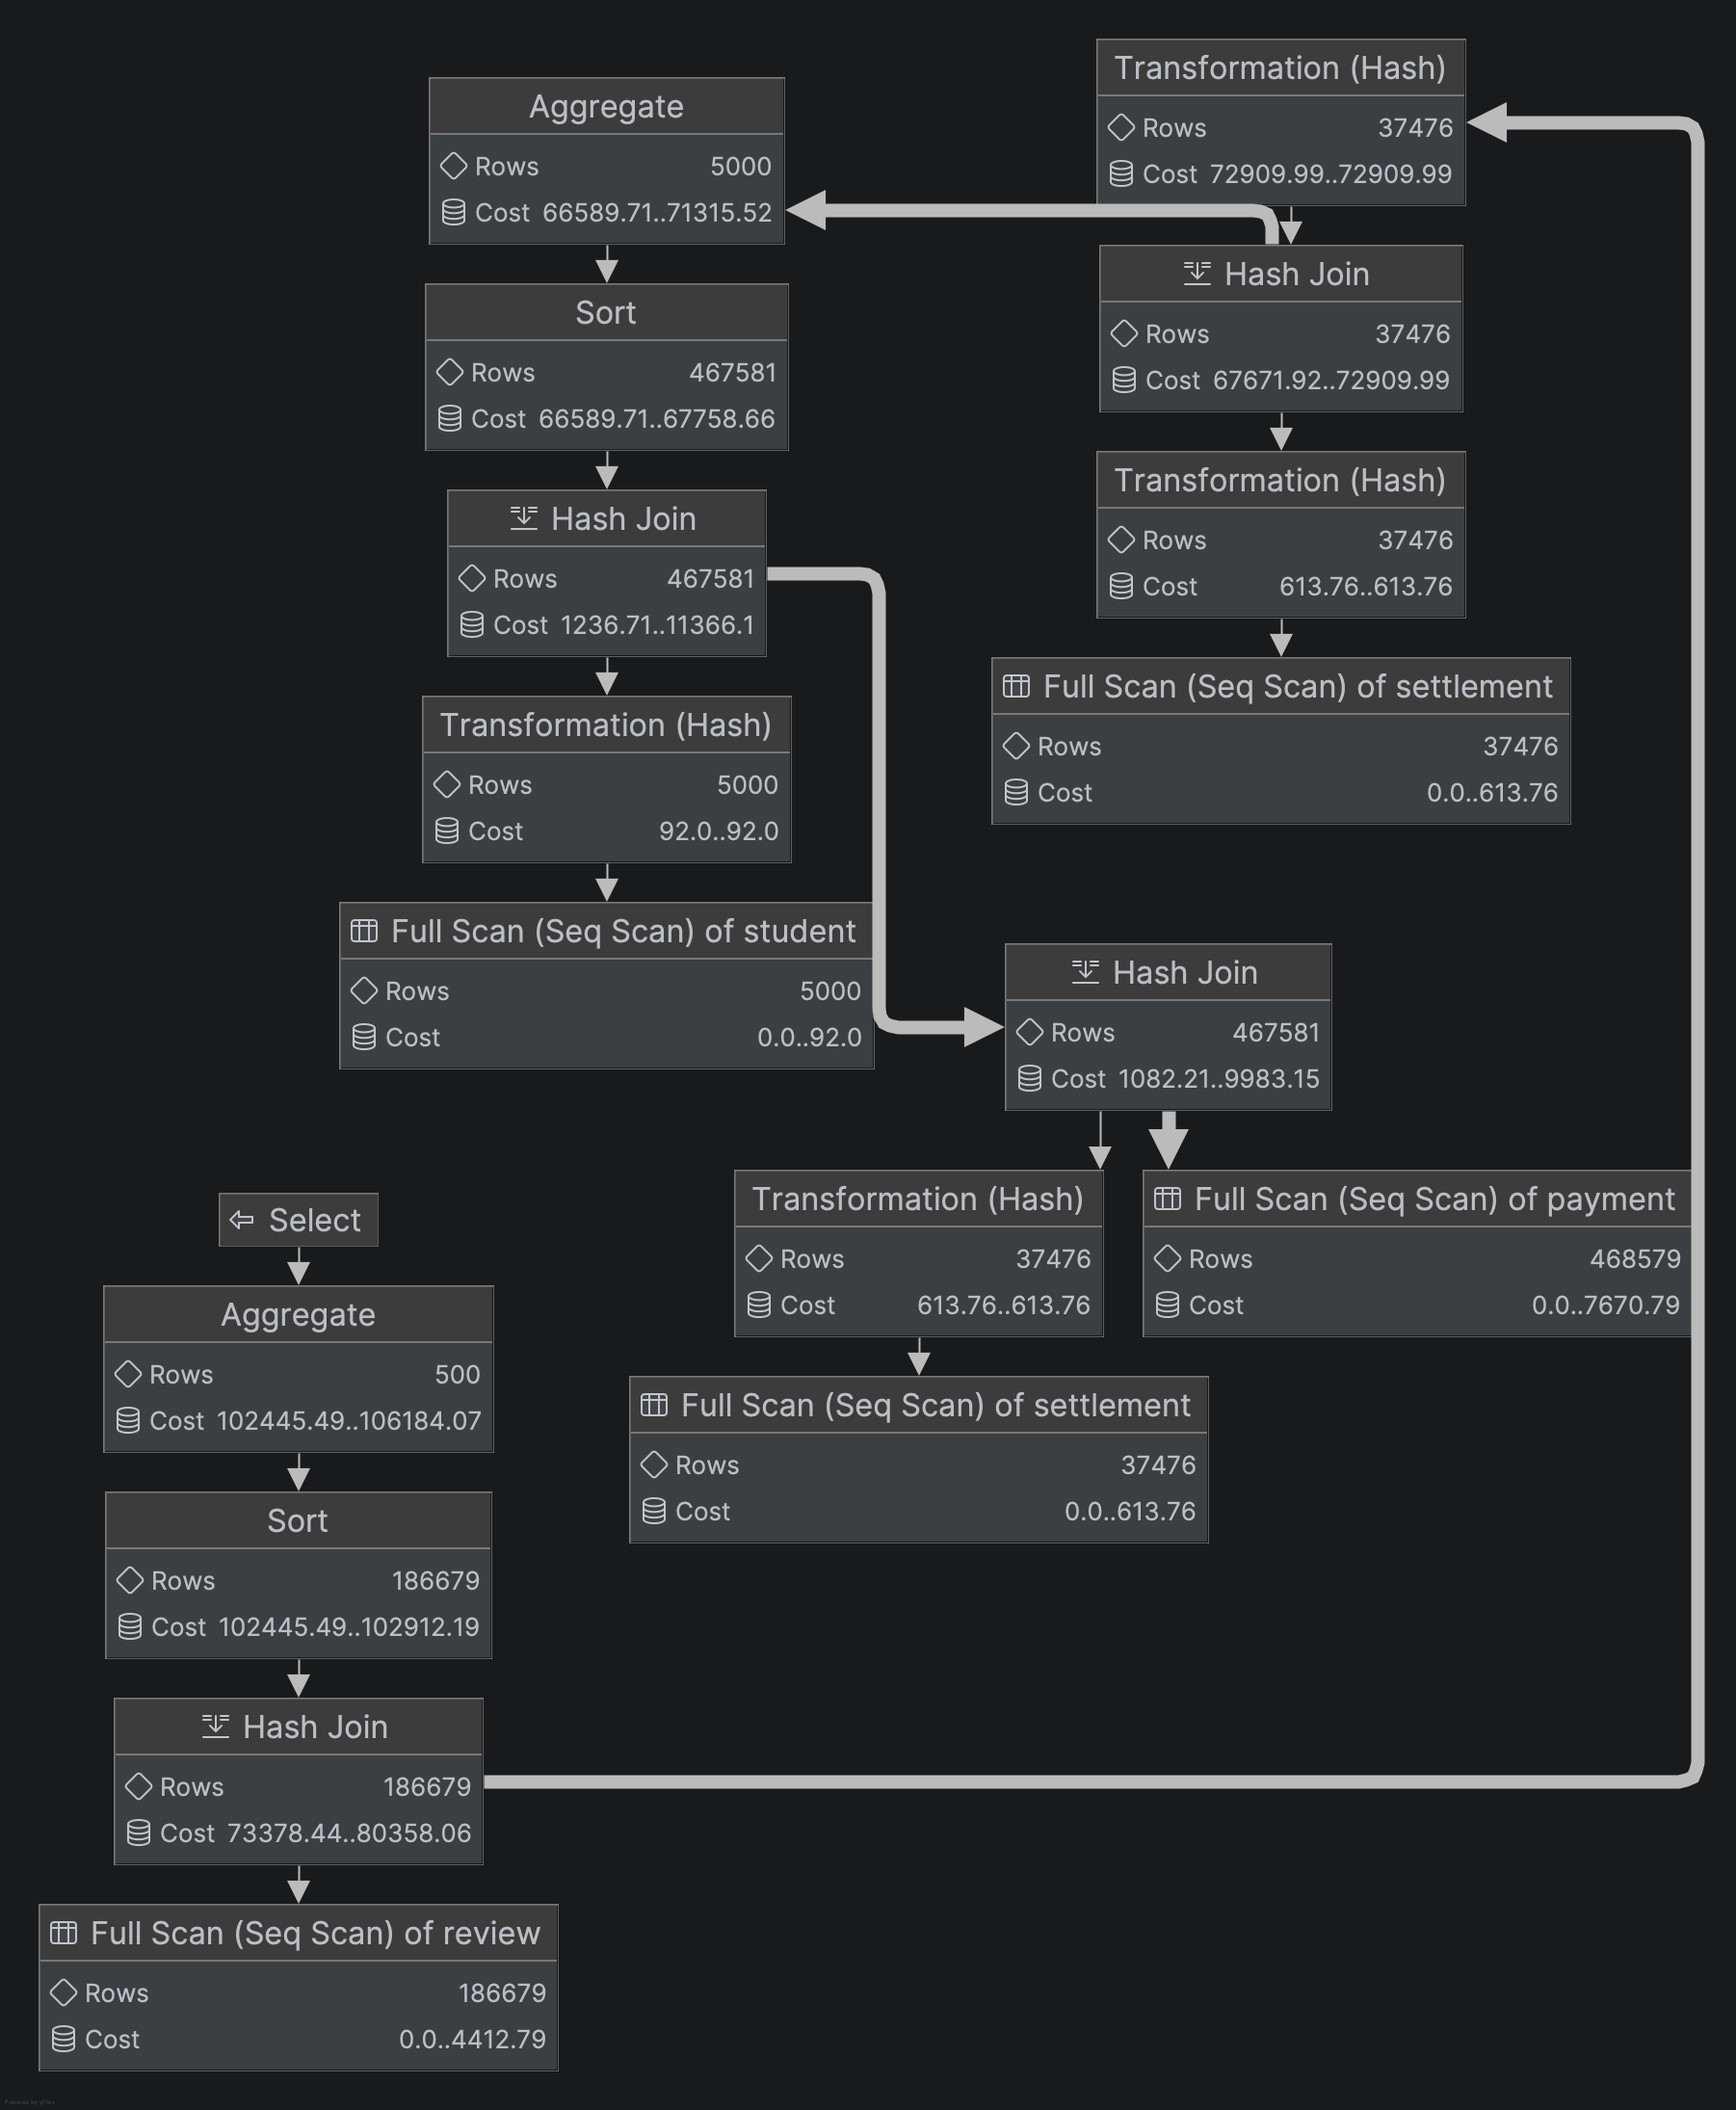
\includegraphics[width=0.8\textwidth]{figures/view_query2.png}
    \caption{Графическое представление сложного запроса}
    \label{fig:view_query2}
\end{figure}

\subsubsection{Обновляемость представления}
Представление является обновляемым, если оно удовлетворяет требованиям СУБД для выполнения операций \texttt{insert}, \texttt{update} и \texttt{delete}. В частности, представление не должно содержать агрегатных функций, группировки, вычисляемых столбцов и некоторых операций объединения, препятствующих однозначному сопоставлению строк представления со строками исходных таблиц.

В данном представлении используются агрегатные функции \texttt{count()}, которые вычисляют количество поселений и платежей для каждого студента. Кроме того, представление содержит \texttt{gorup by}, необходимое для формирования одной строки с результатами подсчёта для каждого студента. Также для получения данных используются операции \texttt{left join} между таблицами \texttt{student}, \texttt{settlement} и \texttt{payment}.

Таким образом, строки представления являются результатом группировки и агрегации данных нескольких таблиц и не соответствуют однозначно отдельным строкам исходных таблиц. Следовательно, представление \texttt{student\_settlement\_payment\_counts} является необновляемым. Непосредственное выполнение операций \texttt{insert}, \texttt{update} и \texttt{delete} над данным представлением невозможно.

Код, демонстрирующий невозможность непосредственного обновления представления, приведён в листинге~\ref{lst:view_update}.

\begin{lstlisting}[
    language=SQL,
    caption={Проверка обновляемости представления}, 
    label={lst:view_update}]
UPDATE
    student_settlement_payment_counts
SET
    settlement_count = 10
WHERE
    student_id = 1;

INSERT INTO
    student_settlement_payment_counts (
        student_id,
        last_name,
        first_name,
        middle_name,
        settlement_count,
        payment_count
    )
VALUES
    (100, 'Khramov', 'Vlad', 'Dmitry', 5, 3);
\end{lstlisting}